\documentclass[dvipdfmx]{beamer}
\AtBeginShipoutFirst{\special{pdf:tounicode EUC-UCS2}}

\usetheme{Madrid}
\usecolortheme{default}
\setbeamerfont{frametitle}{size=\large,series=\bfseries}
\setbeamertemplate{navigation symbols}{}
\setbeamertemplate{footline}[frame number]
\setbeamertemplate{section in toc}[circle]
\setbeamertemplate{blocks}[rounded][shadow=true]

\definecolor{character}{RGB}{0,0,0} %文字
\definecolor{background}{RGB}{245,245,245} %背景
\setbeamercolor{Normal text}{bg=background, fg=character}

\definecolor{mathFormula}{RGB}{53,121,53} %数式
\setbeamercolor{math text}{fg=mathFormula}

\definecolor{alertColor}{RGB}{255,70,70} %alert
\setbeamercolor{alerted text}{fg=alertColor}

\definecolor{blockAlertColor}{RGB}{0,0,0} %alertblock内の文字
\setbeamercolor{block body alerted}{fg=blockAlertColor}

\definecolor{headColor}{RGB}{52,38,89} %見出しカラー
\definecolor{bodyColor}{RGB}{240,240,240} %block背景色
\setbeamercolor{structure}{fg=headColor}
\setbeamercolor{subsection in toc}{fg=headColor}
\setbeamercolor{block body}{bg=bodyColor}

\usepackage[absolute,overlay]{textpos}
\setbeamercovered{dynamic}
%\usepackage[colorgrid,gridunit=pt,texcoord]{eso-pic}


% \mathversion{bold}
% \usefonttheme[onlymath]{serif}
% 文字フォント設定
% \setbeamertemplate{blocks}[rounded] % Blockの影を消す
% \mathversion{bold} %数式を太字に
\usefonttheme{professionalfonts}% 数式用フォント
\setbeamertemplate{items}[ball] % itemize 変更
\renewcommand{\kanjifamilydefault}{\gtdefault}  % 日本語をゴシック体に
\renewcommand{\familydefault}{\sfdefault} %英字をサンセリフに
\newcommand{\argmin}{\mathop{\rm arg~min}\limits}
%\renewcommand{\familydefault}{\rmdefault} %英字をローマンに
%\setbeamertemplate{section in toc}[square] %目次を球体から四角へ
% \newtheorem{remark}[theorem]{Remark}
% \newtheorem{observation}[theorem]{Observation}


\title{並列機械モデルにおける\\最大待ち時間最小化問題の計算論的分析}
\author{15713004 天本 祐希}
\institute{宋研究室}
\date{2018年2月6日}

%%%%%%%%%%%%%%%%%%%%%%%%%%%%%%%%%%%%%%%%%%%%%%%%%%%%%%%%%%%%%%%%%%%
\AtBeginSection[]{
\begin{frame}{目次}
  \tableofcontents[currentsection,currentsubsection,sectionstyle=show/shaded]
  \end{frame} %目次スライド
  }
  \AtBeginSubsection[]{
  \begin{frame}{目次}
    \tableofcontents[currentsection,currentsubsection,sectionstyle=show/shaded]
  \end{frame}
  }
  %%%%%%%%%%%%%%%%%%%%%%%%%%%%%%%%%%%%%%%%%%%%%%%%%%%%%%%%%%%%%%%%%%%
  \begin{document}
  \maketitle
  %%%%%%%%%%%%%%%%%%%%%%%%%%%%%%%%%%%%%%%%%%%%%%%%%%%%%%%%%%%%%%%%%%%
  \begin{frame}{目次}
    \tableofcontents
    \end{frame} %目次スライド
    \section{研究背景と目的}
    \begin{frame}{研究背景と目的:受注生産方式における生産計画の流れ}
      \begin{block}{受注生産方式とは}
        顧客注文を受けてから,その受注製品の生産を全体の生産計画に組み込むため,\alert{どの製造工場}で\alert{いつ製造}するかを決定する.
        \begin{itemize}
          \item 例えば,高級自動車メーカー,システムインテグレーターなど.
        \end{itemize}
      \end{block}

      \begin{figure}[h]
        \centering
        \includegraphics<1>[width=12cm]{figure/car1.pdf}
        \includegraphics<2>[width=12cm]{figure/car2.pdf}
        \includegraphics<3>[width=12cm]{figure/car3.pdf}
        \includegraphics<4>[width=12cm]{figure/car4.pdf}
      \end{figure}
    \end{frame}

    \begin{frame}{研究背景と目的:スケジューリング問題との対応}
      \begin{block}{受注生産方式における問題点}
        製造工場の数と受注状況によって,受注から製造開始までの\alert{待ち時間}が長くなり,顧客満足度の低下や注文のキャンセルなどに繋がる.
      \end{block}
      \begin{itemize}
        \setlength{\leftskip}{-5mm}
        \item 待ち時間を短縮するための生産計画を立てることは重要な課題である.
      \end{itemize}

      \begin{block}{スケジューリング問題との対応}
        各注文を\alert{ジョブ},受注日時を\alert{処理開始可能時刻},製造期間を\alert{処理時間}と対応させることで,受注生産方式における生産計画を\alert{待ち時間}を目的関数とするスケジューリング問題として捉えた.
      \end{block}

      \begin{block}{研究目的}
        上記の問題を\alert{最大待ち時間最小化問題}として定式化し,
        \begin{itemize}
          \setlength{\leftskip}{-2mm}
          \item 問題の計算複雑さを明らかにする.
          \item 問題の計算複雑さを踏まえて,解法の提案を行う.
        \end{itemize}
      \end{block}

    \end{frame}
    %%%%%%%%%%%%%%%%%%%%%%%%%%%%%%%%%%%%%%%%%%%%%%%%%%%%%%%%%%%%%%%%%%%
    \section{諸定義}
    \begin{frame}{諸定義:機械モデル}
      \begin{block}{機械モデル}
        \begin{itemize}
          \item \alert{単一機械モデル}
          \begin{itemize}
            \item 1 つの機械で処理を行う.
            \begin{itemize}
              \item 1 つの製造工場で製造する.
            \end{itemize}
          \end{itemize}
          \item \alert{同一並列機械モデル}
          \begin{itemize}
            \item すべての機械の性能が等しい.
            \begin{itemize}
              \item 複数の製造工場で製造し,各製造工場の設備が同じ.
            \end{itemize}
          \end{itemize}
          \item \alert{一様並列機械モデル}
          \begin{itemize}
            \item 機械ごとに処理速度が異なる.
            \begin{itemize}
              \item 複数の製造工場で製造し,製造工場ごとに設備が異なる.
            \end{itemize}
          \end{itemize}
          \item \alert{無関連並列機械モデル}
          \begin{itemize}
            \item ジョブと機械の組み合わせによって処理時間が異なる.
            \begin{itemize}
              \item 複数の製造工場で製造し,製造工場ごとに異なるメーカーの設備を導入しており,製造する製品によって製造期間が異なる.
            \end{itemize}
          \end{itemize}
        \end{itemize}
      \end{block}
      \begin{itemize}
        \item 無関連並列機械モデルは,すべての機械モデルを含んでいるため,最も一般的な機械モデルである.
      \end{itemize}
    \end{frame}

    \begin{frame}{諸定義:最大待ち時間最小化問題}
      最大待ち時間最小化問題を {\it \alert{S}equencing to minimize maximum \alert{W}aiting \alert{T}ime} の頭文字をとって,\alert{SWT} と表記する.
      \begin{itemize}
        \item 最も一般的な,無関連並列機械モデルにおける SWT を定式化する.
      \end{itemize}
      \begin{block}{インスタンス:$\textcolor{white}{\mathcal{I} = (\mathcal{J}, \mathcal{M}, r, p)}$}
        \begin{itemize}
          \item {ジョブの集合 $\mathcal{J} = \{J_1,J_2,\ldots,J_n\}$}
          \item {無関連機械の集合 $\mathcal{M} = \{M_1,M_2,\ldots,M_m\}$}
          \item {ジョブの処理開始可能時刻を返す関数 $r : \mathcal{J} \to \mathbb{N}$}
          \item {ジョブの処理時間を返す関数 $p : \mathcal{J} \times \mathcal{M} \to \mathbb{N}$}
        \end{itemize}
      \end{block}
      \begin{block}{解:スケジュール $\textcolor{white}{(A,s)}$}
        \begin{itemize}
          \item ジョブの機械への割り当てを返す関数 $A : \mathcal{J} \to \mathcal{M}$.
          \item ジョブの開始時刻を返す関数 $s : \mathcal{J} \to \mathbb{N}$.
          \begin{itemize}
            \item 待ち時間は $r(J) - s(J)$.
          \end{itemize}
        \end{itemize}
      \end{block}
    \end{frame}

    \begin{frame}{諸定義:最大待ち時間最小化問題}
      \begin{block}{制約}
        \begin{itemize}
          \item 各ジョブは処理開始可能時刻以降に処理を開始する.
          \begin{itemize}
            \item $\forall J \in \mathcal{J}\big[s(J) \ge r(J) \big]$
          \end{itemize}
          \item 各機械は同時に複数のジョブを処理しない.
          \item 各ジョブの処理を開始すると,\alert{完了する}まで中断しない.
          \begin{itemize}
            \item {$\forall J, J' \in \mathcal{J}\ \Big[ \big[J\ne J' \land A(J) = A(J')\big] \Rightarrow \textcolor{blue}{\big[}s(J), \textcolor{red}{s(J)+p(J,A(J))}\textcolor{blue}{\big)} \cap \textcolor{blue}{\big[}s(J'), \textcolor{red}{s(J')+p(J', A(J'))}\textcolor{blue}{\big)} = \emptyset \Big]$}
          \end{itemize}
        \end{itemize}
      \end{block}
      \begin{block}{目的関数:最大待ち時間 $\textcolor{white}{W_{\max}}$}
        \begin{itemize}
          \item ジョブの処理開始可能時刻から処理開始までの待ち時間の最大値.
          \begin{itemize}
            \item $\varphi(A,s) = W_{\max} = {\displaystyle \max_{J \in \mathcal{J}}\{s(J) - r(J)\}}$
          \end{itemize}
        \end{itemize}
      \end{block}
      \begin{itemize}
        \item 最大待ち時間 $W_{\max}$ の最小化を目的とする.
      \end{itemize}
    \end{frame}

    %%%%%%%%%%%%%%%%%%%%%%%%%%%%%%%%%%%%%%%%%%%%%%%%%%%%%%%%%%%%%%%%%%%
    \section{研究成果}
    \subsection{最大待ち時間最小化問題の計算複雑さ}
    \begin{frame}{既存のスケジューリング問題との対応}
      処理開始可能時刻付き最大遅れ時間最小化問題 (SRTD) は,ジョブの納期から処理が完了するまでの遅れ時間の最大値の最小化を目的とするスケジューリング問題である.
      \begin{block}{処理開始可能時刻付き最大遅れ時間最小化問題 (SRTD) との対応}
        \begin{figure}
          \centering
          \includegraphics<1>[width=10cm]{figure/SRTD1.pdf}
          \includegraphics<2->[width=10cm]{figure/SRTD2.pdf}
        \end{figure}
        \vspace{-2mm}
        \begin{itemize}
          \item<2-> 納期を処理開始可能時刻と処理時間の和と設定したとき,SRTD における遅れ時間は\alert{待ち時間}として捉えることができる.
        \end{itemize}
      \end{block}
      \begin{itemize}
        \item<3->SWT は SRTD の\alert{部分問題}であり,
        SRTD は,単一機械モデルにおいて\alert{強 NP 困難}であることが示されている[Garey \& Johnson(1990)]が,SWT の計算複雑さは明らかでない.
      \end{itemize}
    \end{frame}

    \begin{frame}{多項式時間還元の流れ}
      SWT の NP 完全性を示すため,NP 完全であることが知られている {\sc 3-SATISFIABILITY (3-SAT)} から\alert{多項式時間還元}を行う.
      \begin{tabular}{cc}
        \begin{minipage}[]{0.6\hsize}
          \begin{block}{多項式時間還元}
            問題 $A$ の任意のインスタンスを,別の問題 $B$ のあるインスタンスに多項式時間で判定結果が一致するように変換できるとき,
            \begin{center}
              「$A$ は $B$ に多項式還元可能」という.
            \end{center}
            $B$ の解法を用いて,$A$ も解くことができるため,$B$ は $A$ と同等か,それ以上難しい.
          \end{block}
        \end{minipage}
        \begin{minipage}[]{0.4\hsize}
          \begin{figure}[h]
            \centering
            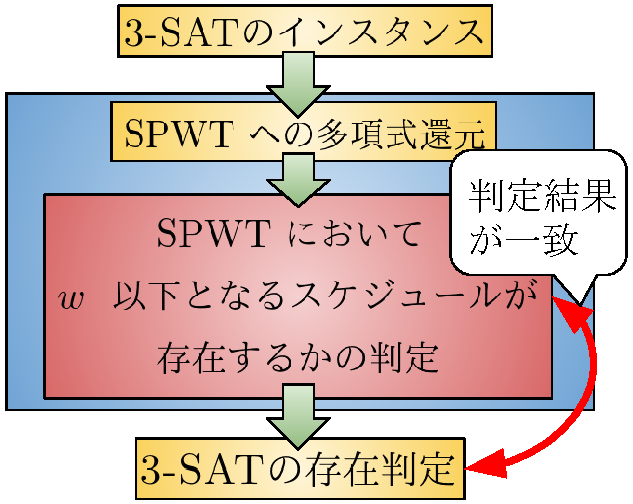
\includegraphics[width=4.5cm]{figure/reduction.pdf}
          \end{figure}
        \end{minipage}
        \vspace{5mm}
      \end{tabular}
      \vspace{-7mm}
      \begin{block}{}
        {\sc 3-SAT} は決定問題の 1 つで,判定として Yes または No のいずれかを持つ.
        判定結果を同じにするために,問題$B$ を SWT のインスタンスに対して,待ち時間 $w$ 以下となるスケジュールが存在するか,という決定問題として定義し,\alert{待ち時間制約付きスケジューリング問題}と表す.
      \end{block}
    \end{frame}

    \begin{frame}{研究成果:問題の計算複雑さ}
      \begin{alertblock}{成果 1}
        無関連並列機械モデルにおいて,機械数が入力の一部の場合,SWT が NP 困難であることを明らかにした.
        \begin{itemize}
          \item NP 完全であることが知られている {\sc 3-SAT} から待ち時間制約付きスケジューリング問題に多項式還元できることを示した.
        \end{itemize}
      \end{alertblock}
      \begin{block}{多項式時間還元のポイント}
        \begin{itemize}
          \item {\sc 3-SAT} のインスタンスにおいて,\alert{各変数に対応する機械}を定義する.
          \item {\sc 3-SAT} のインスタンスにおいて,\alert{各節に対応する機械}を定義する.
          \item \alert{true} に割り当てられたリテラルに対応するジョブは次のジョブを\alert{押し出さない}.
          \item \alert{false} に割り当てられたリテラルに対応するジョブは次の \alert{false} に割り当てられたリテラルに対応するジョブを \alert{$1$ 押し出す}.
        \end{itemize}
      \end{block}
    \end{frame}

    \begin{frame}{研究成果:多項式時間還元のポイント}
      \begin{block}{{\sc 3-SAT} の判定結果が Yes のとき}
        \begin{figure}[h]
          \centering
          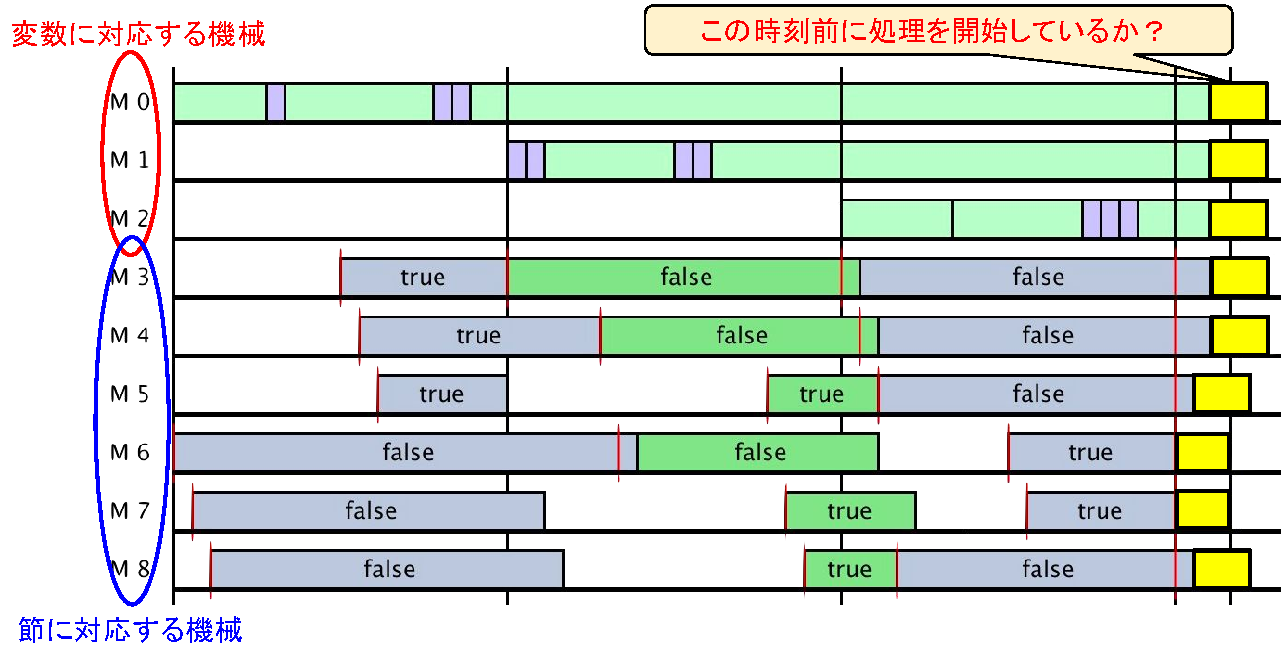
\includegraphics[width=12cm]{figure/reduction1.pdf}
        \end{figure}
      \end{block}
      \begin{itemize}
        \setlength{\leftskip}{-3mm}
        \item {\sc 3-SAT} の判定結果が \alert{Yes} のとき,待ち時間制約付きスケジューリング問題における最大待ち時間が\alert{2 以下}となるスケジュールが\alert{存在する}.
      \end{itemize}
    \end{frame}

    \begin{frame}{研究成果:多項式時間還元のポイント}
      \begin{block}{{\sc 3-SAT} の判定結果が No のとき}
        \begin{figure}[h]
          \centering
          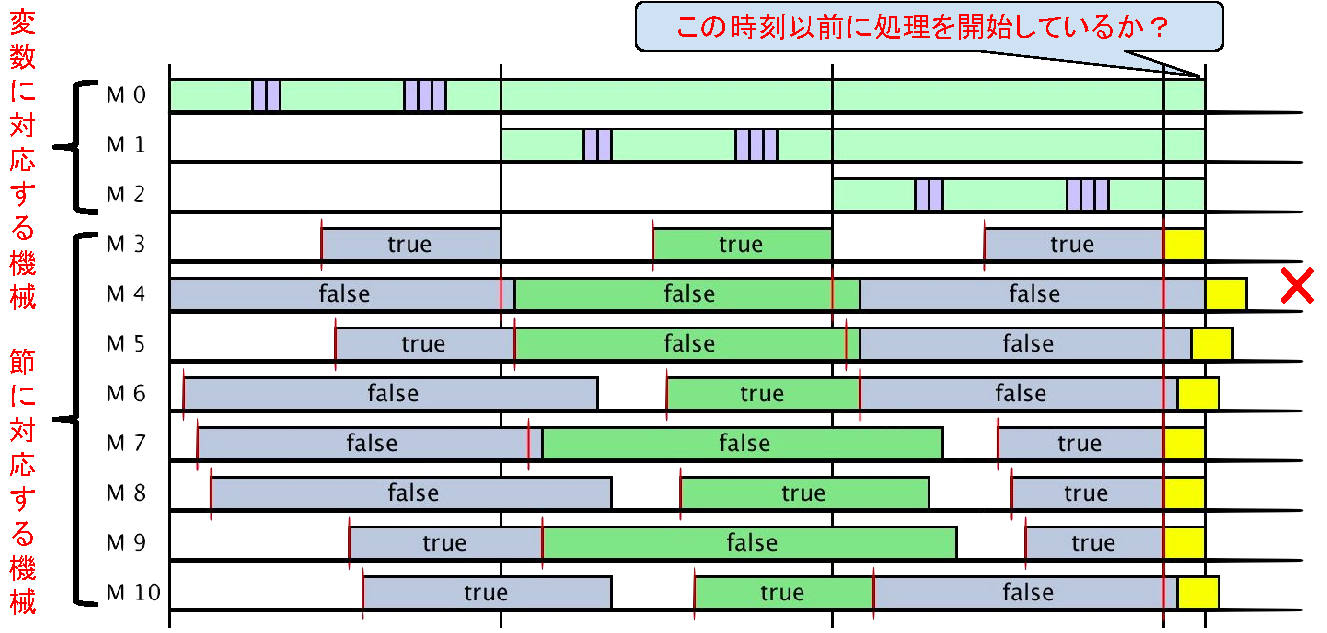
\includegraphics[width=12cm]{figure/reduction2.pdf}
        \end{figure}
      \end{block}
      \begin{itemize}
        \setlength{\leftskip}{-3mm}
        \item {\sc 3-SAT} の判定結果が \alert{No} のとき,待ち時間制約付きスケジューリング問題における最大待ち時間が\alert{2 以下}となるスケジュールが\alert{存在しない}.
      \end{itemize}
    \end{frame}

    \begin{frame}{研究成果:問題計算複雑さ}
      \begin{block}{多項式時間還元の結果}
        待ち時間制約付きスケジューリング問題における最大待ち時間が,
        \begin{itemize}
          \item {\sc 3-SAT} の判定結果が \alert{Yes} のとき,\alert{2 以下},
          \item {\sc 3-SAT} の判定結果が \alert{No} のとき,\alert{3 以上},
        \end{itemize}
        となるスケジュールが存在する.
      \end{block}
      無関連並列機械モデルにおいて機械数が入力の一部の場合,SWT が NP 困難である限り,近似率 $1.5$ 未満の定数近似アルゴリズムは存在しない.
      \begin{alertblock}{成果 1 のまとめ}
        SWT が NP 困難であることを示した.NP 困難な問題に対する効率的な解法は発見されていないため,最適解を求めるために,解の全列挙に基づいた解法が必要である.
      \end{alertblock}
    \end{frame}

    \subsection{厳密解法の提案と実験的評価}
    \begin{frame}{研究成果:厳密解法の提案}
      \begin{alertblock}{成果 2}
        同一並列機械モデルにおける SWT に対し,分割生成アルゴリズムおよび分枝限定法に基づいた厳密解法の開発と計算時間の分析を行った.
      \end{alertblock}
      \begin{block}{分割生成アルゴリズムの改良}
        \begin{itemize}
          \item \alert{分割の要素数 = 機械数} となる分割のみ生成するように改良.
          \begin{itemize}
            \item 考慮する分割の数を減らすことができる.
          \end{itemize}
        \end{itemize}
      \end{block}
      \begin{block}{分枝限定法の改良}
        \begin{itemize}
          \item SRTD の\alert{部分問題に対する多項式アルゴリズム}の概念を導入.
          \begin{itemize}
            \item 列挙する実行可能解を減らすことができる.
          \end{itemize}
        \end{itemize}
      \end{block}
      \begin{block}{上記以外の改良}
        \begin{itemize}
          \item 各機械におけるジョブ集合のコストの降順で,探索を始める.
          \begin{itemize}
            \item 各分割における探索初期段階で,探索の中断を判定できる.
          \end{itemize}
        \end{itemize}
      \end{block}
    \end{frame}

    \begin{frame}{研究成果:厳密解法の実験的評価}
      機械数 5 における計算時間の比較.ただし,計算時間の単位はミリ秒.
      \begin{itemize}
        \item 分割生成アルゴリズムの改良前と,改良後の計算時間の比較
        \begin{tabular}{|c|c|c|c|c|c|} \hline
          ジョブ数 & 10 & 11 & 12 & 13 & 14 \\ \hline \hline
          改良前 & 553 & 3,463 & 30,271 & 240,917 & 3,121,089 \\ \hline
          改良後 & 146 & 943 & 7,576 & 40,748 & 249,759  \\ \hline
          削減率 & 73\% & 72\% & 75\% & 83\% & \alert{92\%} \\ \hline
        \end{tabular}
        \item 分枝限定法の改良前と,改良後の計算時間の比較
        \begin{tabular}{|c|c|c|c|c|c|c|} \hline
          ジョブ数 & 10 & 11 & 12 & 13 & 14 & 15\\ \hline \hline
          改良前 & 313 & 1,709 & 9,758 & 54,966 & 295,287 & 1,668,411 \\ \hline
          改良後 & 168 & 971 & 6,887 & 43,903 & 225,043 & 1,301,890 \\ \hline
          削減率 & 46\% & 43\% & 30\% & 20\% & 23\% & \alert{22\%} \\ \hline
        \end{tabular}
      \end{itemize}
      \begin{alertblock}{成果 2 のまとめ}
        改良により,計算時間を大幅に減らすことを可能にしたが,全探索では,ジョブの増加に伴い計算時間が指数的に増大する.そのため,より大きいインスタンスに対しては,ヒューリスティックの開発が必要である.
      \end{alertblock}
    \end{frame}

    \subsection{ヒューリスティックの提案とその精度評価}
    \begin{frame}{既存のスケジューリング問題との対応}
      JIT ジョブ荷重和最大化問題 (SJIT) は,納期以前に処理を完了したジョブの荷重和の最大化を目的とするスケジューリング問題である.
      \begin{block}{JIT ジョブ荷重和最大化問題 (SJIT) との対応}
        SJIT において,各ジョブを JIT で処理可能なとき,各ジョブは納期ちょうどで処理が完了する.つまり,各ジョブの待ち時間は $0$ である.
        \vspace{-2mm}
        \begin{figure}[h]
          \centering
          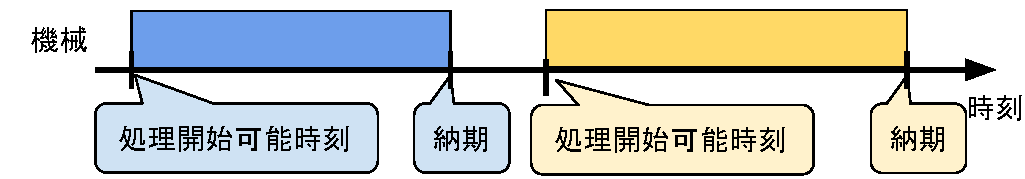
\includegraphics[width=10cm]{figure/SJIT1.pdf}
        \end{figure}
        \vspace{-2mm}
        SJIT において,各ジョブを JIT で処理できるとき,処理開始可能時刻の昇順で処理することで最適解が求まる.[Cepek \& Sung(2004)]
      \end{block}
      \begin{block}{}
        SWT において,各ジョブの待ち時間が $0$ のとき,処理開始可能時刻の昇順で処理することで最適解が求まる.したがって,貪欲アリゴリズムに基づいたヒューリスティックの開発を行う.
      \end{block}
    \end{frame}

    \begin{frame}{研究成果:ヒューリスティックの提案}
      \begin{alertblock}{成果 3}
        同一並列機械モデルにおける SWT に対して,貪欲アルゴリズムに基づいたヒューリスティックの開発と解法に対する実験的評価を行った.
      \end{alertblock}
      \begin{block}{ヒューリスティックの評価}
        本研究では,ヒューリスティックから得られた解における最大待ち時間と最適解における最大待ち時間の比に基づき評価を行った.
        $${\displaystyle \text{競合比} = \frac{\text{ヒューリスティックから得られた解における最大待ち時間}\cdots A}{\text{最適解における最大待ち時間}\cdots B}}$$
      \end{block}
      \begin{alertblock}{成果 3 のまとめ}
        ヒューリスティックは,競合比が最大 $24$ となった.
        また,最適解における最大待ち時間が $0$ のとき,ヒューリスティックは常に最適解を返す.
      \end{alertblock}
    \end{frame}
    %%%%%%%%%%%%%%%%%%%%%%%%%%%%%%%%%%%%%%%%%%%%%%%%%%%%%%%%%%%%%%%%%%%
    \section{まとめと今後の課題}
    \begin{frame}{まとめと今後の課題}
      \begin{block}{まとめ}
        \begin{itemize}
          \item 無関連並列機械モデルにおいて機械数が入力の一部の場合,SWT が NP 困難であることを明らかにした.
          \begin{itemize}
            \item 近似率 1.5 未満の定数近似ができないことを明らかにした.
          \end{itemize}
          \item SWT に対する厳密解法とヒューリスティックを開発し,実験的評価を行った.
        \end{itemize}
      \end{block}
      \begin{alertblock}{今後の課題}
        \begin{itemize}
          \item 無関連並列機械モデル以外の機械モデルにおける SWT の計算複雑さを明らかにし,問題の難しさに影響を与える特徴を分析する.
          \item {\sc 3-SAT} からの還元手法を工夫して,{\sc 3-SAT} の存在判定が Yes のとき,No のときの待ち時間制約付きスケジューリング問題における最大待ち時間の比を調整する.
          \begin{itemize}
            \item 上記の比を大きくすることができれば,近似率がその比未満の定数近似アルゴリズムが存在しないことを保証できる.
          \end{itemize}
          \item 上記の結果に基づき,近似アルゴリズムを開発する.
        \end{itemize}
      \end{alertblock}
    \end{frame}
    %%%%%%%%%%%%%%%%%%%%%%%%%%%%%%%%%%%%%%%%%%%%%%%%%%%%%%%%%%%%%%%%%%%
    \begin{frame}

    \end{frame}
    %%%%%%%%%%%%%%%%%%%%%%%%%%%%%%%%%%%%%%%%%%%%%%%%%%%%%%%%%%%%%%%%%%%
    \begin{frame}{付録:${\textcolor{white}{\mbox {\sc 3-SAT}}}$ の定式化}
      \textsc{3-SATISFIABILITY (3-SAT) } は決定問題の 1 つで,この問題は NP 完全であることが知られている.
      \begin{block}{\textsc{3-SATISFIABILITY}}
        \begin{description}
          \item[インスタンス:] $(X,H)$
          \vspace{-2mm}
        \end{description}
        \begin{itemize}
          \item ブール型の変数集合 $X=\{x_1,x_2,\dots ,x_n\}$
          \begin{itemize}
            \item リテラルの集合 $L_X = X \cup \{\bar x \mid x \in X\}$
            \begin{itemize}
              \item $X$ と $X$ の各要素の論理否定をとった変数の集合
            \end{itemize}
          \end{itemize}
          \item 3 つのリテラルからなる節 $h$ の集合 $H$
          \begin{itemize}
            \item $H \subseteq 2^{L_X}$ s.t. $\forall h \in H \big[|h| = 3\big]$
          \end{itemize}
        \end{itemize}
        \begin{description}
          \setlength{\leftskip}{-8mm}
          \item[問題:] 以下を満たす真理値割り当て $f : X \to \{0,1\}$ が存在するか?
        \end{description}
        \vspace{-1mm}
        $$\displaystyle \bigwedge_{h \in H} \bigg(\bigvee_{x \in h}f(x) \lor \bigvee_{\bar x \in h}\lnot f(x) \bigg) = 1$$
        \vspace{-1mm}
      \end{block}
    \end{frame}

    \begin{frame}{付録:${\textcolor{white}{\mbox {\sc 3-SAT}}}$ の例}
      \begin{exampleblock}{${\textcolor{white}{\mbox {\sc 3-SAT}}}$ の例}
        \begin{description}
          \item[インスタンス:] $(X,H)$
          \vspace{-2mm}
        \end{description}
        \begin{itemize}
          \item ブール型の変数集合 $X=\{x_1,x_2,x_3\}$
          \begin{itemize}
            \item リテラルの集合 $L_X = \big\{ x_1,x_2,x_3,\bar x_1,\bar x_2,\bar x_3 \big\}$
            \begin{itemize}
              \item $X$ と $X$ の各要素の論理否定をとった変数の集合
            \end{itemize}
          \end{itemize}
          \item 3 つのリテラルからなる節 $h$ の集合 $H$
          \begin{itemize}
            \item $H = \big\{ \textcolor{red}{\{x_1, x_2, \bar x_3\}}, \textcolor{blue}{\{\bar x_1, \bar x_2,x_3\}}\big\}$
            \begin{itemize}
              \item $h_1 = \textcolor{red}{\{x_1, x_2, \bar x_3\}}$, $h_2 = \textcolor{blue}{\{\bar x_1, \bar x_2,x_3\}}$
            \end{itemize}
          \end{itemize}
        \end{itemize}
        \begin{description}
          \setlength{\leftskip}{-8mm}
          \item[問題:] 以下を満たすように $x_1$,$x_2$,$x_3$ を $0$,$1$ で決定できるか?
        \end{description}
        $$(x_1 \lor x_2 \lor \bar x_3) \land (\bar x_1 \lor \bar x_2 \lor  x_3) = 1$$

        $f(x_1) = 1, f(x_2) = 0, f(x_3) = 1$ が存在するので,判定は Yes となる.
      \end{exampleblock}
    \end{frame}

    \begin{frame}{付録:問題の計算複雑さ}
      \begin{block}{還元のポイント}
        \begin{itemize}
          \item {\sc 3-SAT} の判定結果が \alert{Yes} のとき,待ち時間制約付きスケジューリング問題における最大待ち時間は \alert{2 以下}になる .
          \item {\sc 3-SAT} の判定結果が \alert{No} のとき,待ち時間制約付きスケジューリング問題における最大待ち時間は \alert{3 以上}になる .
        \end{itemize}
      \end{block}
      \begin{block}{表記の導入}
        {\sc 3-SAT} のインスタンス を $X = \{x_1,\ldots,x_n\}$ と $H = \{h_1,\ldots,h_{\lambda}\}$ からなる 2 項組 $(X,H)$ とする.
        $(X,H)$ に基づき表記を導入する.
        \begin{itemize}
          \item $\forall i \in \{1,\ldots,n\},~\alpha_i = |\{h \in H \mid x_i \in h\}|$
          \begin{itemize}
            \item $H$ において,$x_i$ が現れる回数を表す自然数を $\alpha_i$ とする.
          \end{itemize}
          \item $\forall i \in \{1,\ldots,n\},~\beta_i = |\{h \in H \mid \bar x_i \in h\}|$
          \begin{itemize}
            \item $H$ において,$\bar x_i$ が現れる回数を表す自然数を $\beta_i$ とする.
          \end{itemize}
          \item $\mathcal{A} = {\displaystyle \sum_{i \in \{1,\ldots,n\}}\alpha_i}$,$\mathcal{B} = {\displaystyle \sum_{i \in \{1,\ldots,n\}}\beta_i}$
        \end{itemize}
      \end{block}
    \end{frame}

    \begin{frame}{付録:問題の計算複雑さ}
      $2(\mathcal{A} + \mathcal{B}) + n + \lambda$ 個のジョブ $\mathcal{J}$ を $n + \lambda$ 個の無関連機械で処理する.
      \begin{block}{変換した待ち時間制約付きスケジューリング問題のインスタンス}
        $2(\mathcal{A} + \mathcal{B}) + \lambda$ 個のジョブ
        \begin{itemize}
          \item 各 $i \in \{1,\ldots,n\}$ における変数 $x_i$ からなるリテラル $x_i$,$\bar x_i$ に対応するジョブの集合を $\mathcal{J}^t(i)$,$\mathcal{J}^f(i)$ とする.それぞれの要素数は,$x_i$ と $\bar x_i$ が $H$ に現れた回数,つまり,$|\mathcal{J}^t(i)| = |\mathcal{J}^f(i)| = \alpha_i + \beta_i$.
          \item $n + \lambda$ は,$X$ と $H$ の要素数.各変数と各節に対応する機械に割り当てる用のダミージョブ.
        \end{itemize}
        $n + \lambda$ 個の機械
        \begin{itemize}
          \item $n$ は $X$ の要素数.
          各変数に対応する機械が 1 台ある.
          \item $\lambda$ は $H$ の要素数.
          各節に対応する機械が 1 台ずつある.
        \end{itemize}
      \end{block}
      \begin{itemize}
        \item $f(x_i) = 1$ のとき,
        $\mathcal{J}^f(i)$ を機械 $i$ に割り当てる.
        \item $f(x_i) = 0$ のとき,
        $\mathcal{J}^t(i)$ を機械 $i$ に割り当てる.
      \end{itemize}
    \end{frame}

    \begin{frame}{付録:問題の計算複雑さ}
      \begin{block}{各機械 ${\textcolor{white}{i \in \{1,\ldots,n\}}}$ に対応するジョブのスケジュール}
        \begin{figure}[h]
          \centering
          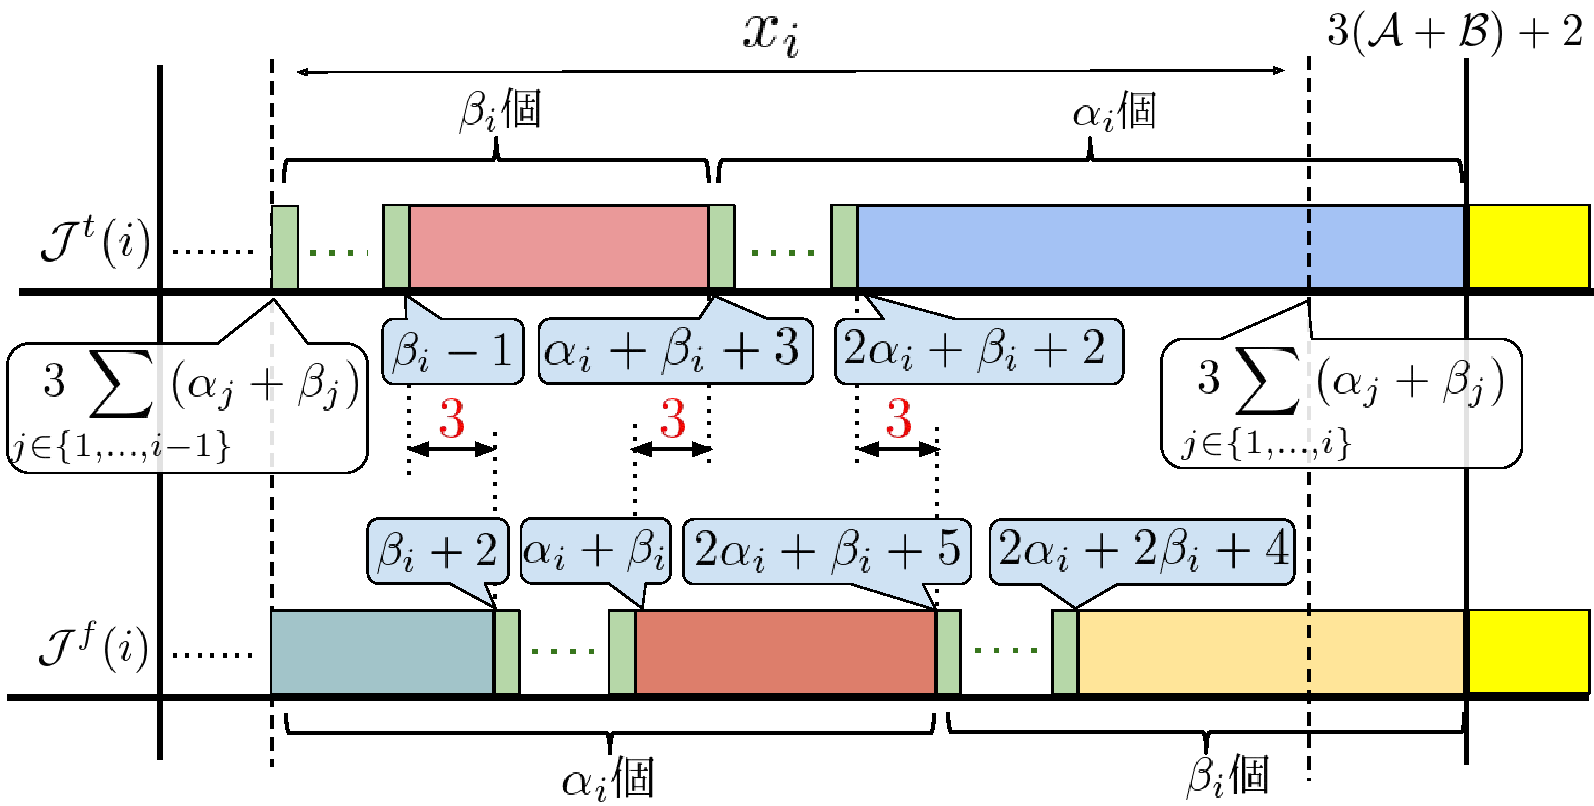
\includegraphics[width = 10.5cm]{figure/3SAT4.pdf}
        \end{figure}
      \end{block}
      \begin{itemize}
        \item $x_i$ と $\bar x_i$ に対応するジョブの集合 $\mathcal{J}^t(i)$ と $\mathcal{J}^f(i)$ におけるジョブ間の処理開始可能時刻の差を $3$ に設定する.
        \item $\mathcal{J}^t(i)$ の要素 $J^t(i)$ と $\mathcal{J}^f(i)$ の要素 $J^f(i)$ が機械 $i$ に同時に割り当てられないように,上記の差を設けている.
      \end{itemize}
    \end{frame}

    \begin{frame}{付録:問題の計算複雑さ}
      \begin{block}{各機械 ${\textcolor{white}{\ell \in \{n + 1,\ldots,n + \lambda\}}}$ に対応するジョブのスケジュール}
        $h_{\ell - n} = \{x_i, x_j, x_k\}$ のとき,
        \begin{description}
          \setlength{\leftskip}{-12mm}
          \item[$S$:]
          $f(x_i) = 1, f(x_j) = 0, f(x_k) = 0$ のとき.
          %機械 $\ell$ に割り当てるジョブは,$J_i \in \mathcal{J}^t(i)$,$J_j \in \mathcal{J}^f(j)$,$J_k \in \mathcal{J}^f(k)$ とダミージョブ $J_d$.
          \item[$S'$:]
          $f(x_i) = 0, f(x_j) = 0, f(x_k) = 0$ のとき.
          %機械 $\ell$ に割り当てるジョブは,$J_i \in \mathcal{J}^f(i)$,$J_j \in \mathcal{J}^f(j)$,$J_k \in \mathcal{J}^f(k)$ とダミージョブ $J_d$.
        \end{description}
        \vspace{-5mm}
        \begin{figure}[h]
          \centering
          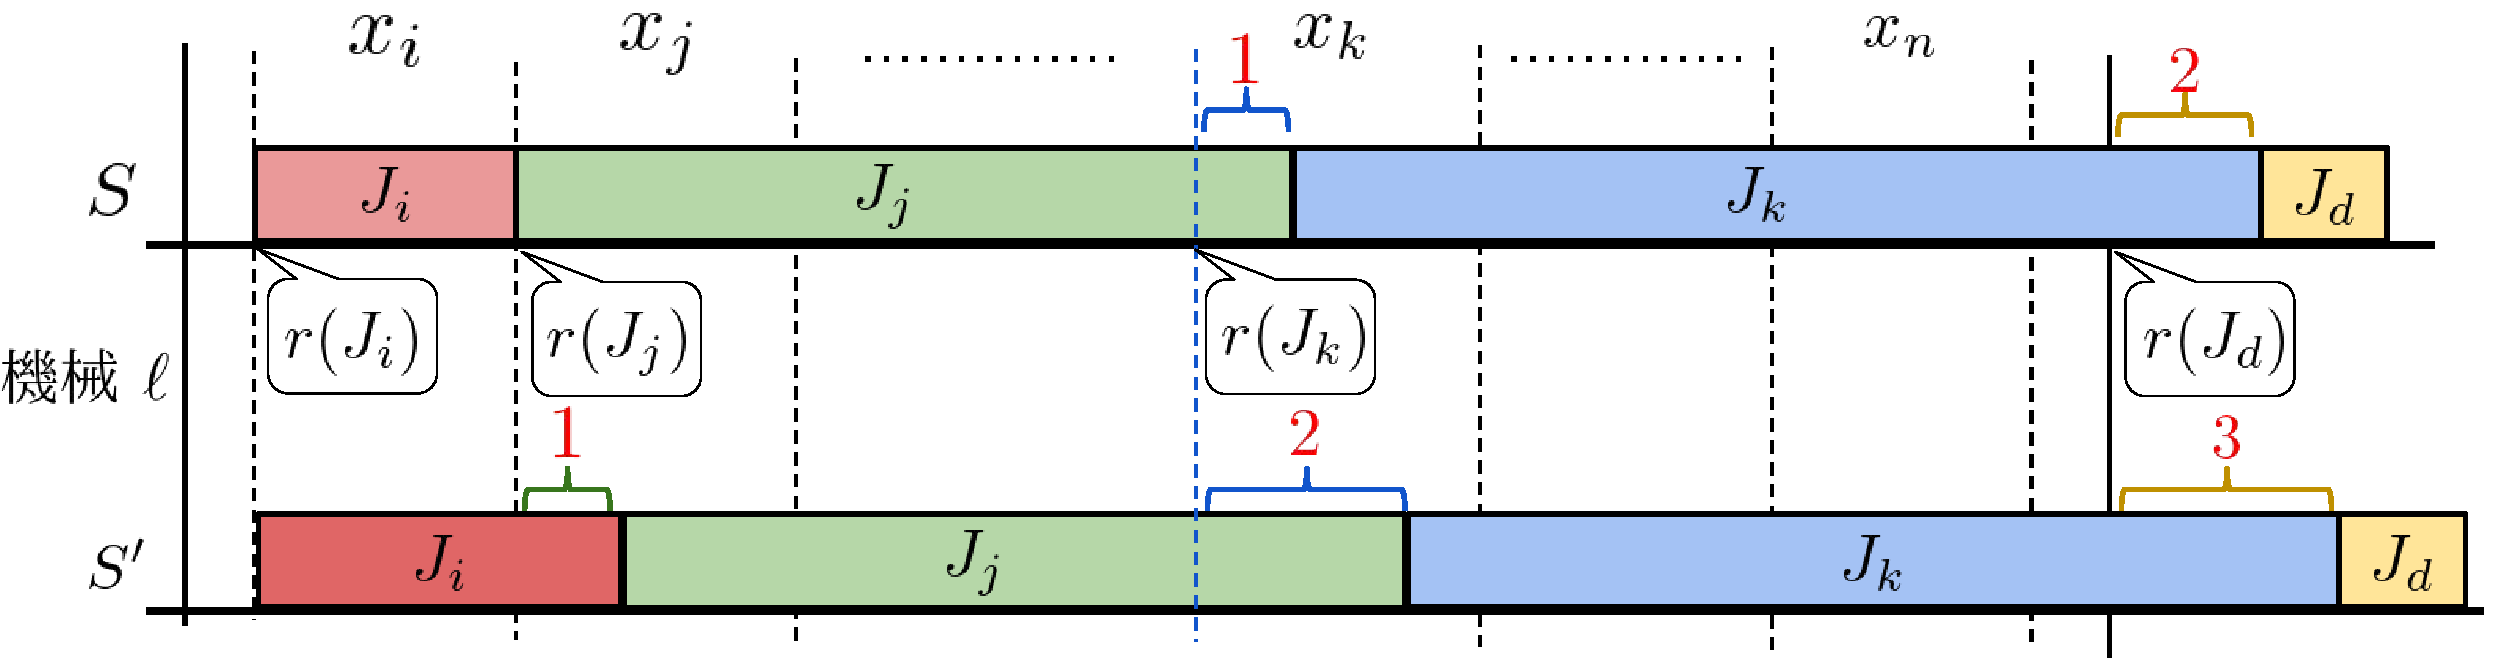
\includegraphics[width=12cm]{figure/3SAT6.pdf}
        \end{figure}
      \end{block}
      \begin{itemize}
        \item $1$ に割り当てられたリテラルに対応するジョブは,
        \begin{itemize}
          \item 次のジョブの処理開始可能時刻 - 自身の処理開始可能時刻
        \end{itemize}
        \item $0$ に割り当てられたリテラルに対応するジョブは,
        \begin{itemize}
          \item 次のジョブの処理開始可能時刻 - 自身の処理開始可能時刻 + 1
        \end{itemize}
      \end{itemize}
    \end{frame}

    \begin{frame}{付録:多項式還元の例(特殊なケース)}
      \begin{block}{特殊なケースにおけるインスタンスの作り方}
        例えば,$X = \{x_1,x_2,x_3\}$,$H = \big\{{\textcolor{red}{\{x_1,x_2,x_3\}}},{\textcolor{blue}{\{\bar x_1, \bar x_2, \bar x_3\}}}\big\}$ のとき,
        \begin{itemize}
          \item
          各 $i \in \{1,2,3\}$ に対して,$\alpha_i$,$\beta_i$ は 3 以下である.
          \item
          このとき,各 $i \in \{1,2,3\}$ に対して,$\alpha_i$,$\beta_i$ は 3 以上となるように,ダミーの節を作る.以下の通り.
        \end{itemize}
        \begin{equation}
          \begin{split}
            H &= \big\{
            {\textcolor{red}{\{x_1,x_2,x_3\}}},
            {\textcolor{red}{\{x_1,x_2,x_3\}}},
            {\textcolor{red}{\{x_1,x_2,x_3\}}},
            \\ & \qquad\qquad\qquad\qquad\qquad
            {\textcolor{blue}{\{\bar x_1, \bar x_2, \bar x_3\}}},
            {\textcolor{blue}{\{\bar x_1, \bar x_2, \bar x_3\}}},
            {\textcolor{blue}{\{\bar x_1, \bar x_2, \bar x_3\}}}
            \big\} \notag
          \end{split}
        \end{equation}
        \begin{itemize}
          \item 作成したダミー節は,本来 $H$ の要素である節と同じ節を複数個用意したに過ぎない.そのため,真理値割り当てに関係なく,判定結果にも影響しない.
        \end{itemize}
        上記のように,ダミー節を含んだ節の集合を作り,その後,待ち時間制約付きスケジューリング問題のインスタンスへの変換する.インスタンスの変換方法は,前のスライドで記述した通り.
      \end{block}
    \end{frame}

    % \begin{frame}{付録:${\textcolor{white}{\mbox {\sc 3-SAT}}}$ のインスタンスにおける注意点}
    %   \begin{block}{{\sc 3-SAT} のインスタンスにおいて除くケース}
    %     $H$ に現れるリテラルが各変数,もしくは変数の論理否定をとったもののいずれかしか現れないかつ,そのリテラルがすべての節に現れる場合,$H$ を充足する真理値割り当ては常に存在するためこの場合を除く.
    %   \end{block}
    %
    %   \begin{exampleblock}{例:{\sc 3-SAT} のインスタンスにおいて除くケース}
    %     $X = \{x_1,x_2,x_3\}$,
    %     $H = \big\{\{x_1,x_2,\bar x_3\}, \{\bar x_1, \bar x_2, \bar x_3\}\big\}$ のとき,変数 $x_3$ に対応するリテラルは,$\bar x_3$ しか $H$ に現れない.さらに,すべての節に $\bar x_3$ が現れる.
    %     このとき,$f(x_3) = 0$ とすることで,$H$ を充足する真理値割り当てが常に存在する.
    %   \end{exampleblock}
    % \end{frame}

    \begin{frame}{付録:ヒューリスティックのアルゴリズム}
      \begin{block}{貪欲アルゴリズムに基づいた解法}
        \begin{description}
          \setlength{\leftskip}{-10mm}
          \item[入力 :] $I = (\mathcal{J}, \mathcal{M},r,p,C)$
          \item[出力 :] スケジュールの集合 $\mathcal{S}$.
          \begin{description}
            \setlength{\leftskip}{-25mm}
            \item[Step 1.]
            $\mathcal{J}$ を処理開始可能時刻の昇順でソートする.
            \item[Step 2.]
            各 $1 \le i \le n$ における $J_i$ について以下の処理を繰り返す.
            \begin{description}
              \item[Step 2.1.]
              \setlength{\leftskip}{-40mm}
              最小完了時刻を持つスケジュール集合の要素 $S_{M_a} \in \left\{ \displaystyle \argmin_{M \in \mathcal{M}}C(S_M)\right\}$ を 1 つ求める.
              ここで,$S_{M_a} := S_{M_a} \cup J_i$ とする.
            \end{description}
            \item[Step 3.]
            $\mathcal{S} = \{ S_M \mid M \in \mathcal{M}\}$ として,$\mathcal{S}$ を出力する.
          \end{description}
        \end{description}
      \end{block}
    \end{frame}

    \begin{frame}{付録:分割生成アルゴリズムの改良}
      \begin{block}{}
        \uncover<1->{
        \alert{同一並列機械モデル}において,ジョブ $J$ を機械 $1$ に割り当てるのと,機械 $2$ に割り当てることは同じである.
        したがって,ジョブをどの機械に割り当てるかではなく,\alert{どのジョブと同じ機械に割り当てるか}を考える必要がある.
        つまり,同一並列機械モデルにおけるジョブの機械への割り当ては,\alert{ジョブの分割}として捉えることができる.
        }
      \end{block}
      \begin{exampleblock}{例:ジョブ数 3,同一機械数 2 における分割}
        \begin{figure}[h]
          \centering
          \includegraphics<1>[width = 12cm]{figure/rgf1.pdf}
          \includegraphics<2>[width = 12cm]{figure/rgf2.pdf}
          \includegraphics<3>[width = 12cm]{figure/rgf3.pdf}
          \includegraphics<4>[width = 12cm]{figure/rgf4.pdf}
        \end{figure}
      \end{exampleblock}
    \end{frame}

    \begin{frame}{付録:分割生成アルゴリズムの改良部分}
      \begin{block}{表記の導入}
        \begin{itemize}
          \item ジョブ数 $n$,機械数 $m$
          \item 要素数 $n$ の配列 $b$ は分割を表す.
          \item 要素数 $n$ の配列 $b_{\max}$ は 各 $1 \le i \le n$ に対して,$i$ 番目の要素は,それまでのジョブが割り当てられた機械の最大数を格納している.つまり,$b_{\max}[i] = \displaystyle \max_{1\le j \le i - 1}b[j]$
        \end{itemize}
      \end{block}

      \begin{block}{分割生成アルゴリズムの改良部分}
        \begin{description}
          \setlength{\leftskip}{-10mm}
          \item[入力 :] $I = (b, b_{\max}, m)$
          \item[出力 :] 分割 $b$
          \begin{description}
            \setlength{\leftskip}{-25mm}
            \item[Step 1.]
            各 $1 \le i \le n$ に対して,以下の処理を繰り返す.
            \begin{description}
              \setlength{\leftskip}{-40mm}
              \item[Step 1.1.]
              $b_{\max}[n - i] \ge m - i$ のとき,処理を終了する.
              \item[Step 1.2.]
              $b[n - i] := m - i$,$b_{\max}[n - i] := m - i$ とする.
            \end{description}
            \item[Step 2.]
            $b$ を出力する.
          \end{description}
        \end{description}
      \end{block}
    \end{frame}

    \begin{frame}{付録:分割生成アルゴリズムの改良部分}
      \begin{exampleblock}{例:$\textcolor{white}{b = (0,1,0,1)}$,$\textcolor{white}{b_{\max} = (0,1,1,1)}$,$\textcolor{white}{m = 3}$ のとき}
        \begin{description}
          \item[Step 1.]
          $b_{\max}(0,1,1,\textcolor{red}{1} )$ より,$1 < 3 - 1$.
          \item[Step 2.]
          したがって,$b = (0,1,0,2)$,$b_{\max} = (0,1,1,2)$ とする.
          \item[Step 3.]
          $b_{\max}(0,1,\textcolor{red}{1} ,2)$ より,$1 \ge 3 - 2$.
          \item[Step 4.]
          $b$ を出力する.
        \end{description}

      \end{exampleblock}
    \end{frame}

    \begin{frame}{付録:分枝限定法の改良部分}
      \begin{block}{分枝限定法の改良部分}
        \begin{description}
          \setlength{\leftskip}{-10mm}
          \item[入力 :] $I = (\mathcal{J'}, S)$
          \item[出力 :] スケジュール $S$.
          \begin{description}
            \setlength{\leftskip}{-25mm}
            \item[Step 1.]
            各 $1 \le i \le |\mathcal{J'}|$ における $J'_i$ について,以下の処理を繰り返す.
            \begin{description}
              \setlength{\leftskip}{-40mm}
              \item[Step 1.1.]
              $p(J'_i) = {\displaystyle \min_{j \in \{1,\ldots,|\mathcal{J'}|\}}p(J'_j)}$ とする.
              \item[Step 1.2.]
              $S := S \cup J'_i$ とする.
            \end{description}
            \item[Step 2.]
            $S$ を出力する.
          \end{description}
        \end{description}
      \end{block}
      \begin{itemize}
        \item Step 1. で $\mathcal{J'}$ におけるすべてのジョブの処理時間を $\mathcal{J'}$ の中の最小の処理時間に設定している.
        \item 上記の操作により,$\mathcal{J'}$ におけるジョブの本来の処理時間は,設定した処理時間以上である.
        \item このとき,処理開始可能時刻順で処理して得られるスケジュールにおける最大待ち時間は,$\mathcal{J'}$ におけるコストの下限である.
      \end{itemize}
    \end{frame}

    \begin{frame}{付録:分枝限定法の改良}
      \begin{exampleblock}{例:以下のインスタンスにおけるスケジュール生成}
        \begin{tabular}{cc}
          \begin{minipage}[]{0.6\hsize}
            \begin{figure}[h]
              \centering
              \includegraphics<1>[width = 8cm]{figure/BandB1.pdf}
              \includegraphics<2>[width = 8cm]{figure/BandB2.pdf}
            \end{figure}
          \end{minipage}
          \begin{minipage}[c]{0.4\hsize}
            \begin{table}[htb]
              \begin{tabular}{|l|c|r|} \hline
                $\mathcal{J}$ & $r(J)$ & $p(J)$ \\ \hline \hline
                $J_1$ & 2 & 4 \\ \hline
                $J_2$ & 5 & 7 \\ \hline
                $J_3$ & 10 & 15 \\ \hline
              \end{tabular}
            \end{table}
          \end{minipage}
        \end{tabular}
      \end{exampleblock}
      \begin{itemize}
        \uncover<1>{
        \item それまでに割り当てたジョブのスケジュールにおける最大待ち時間がそれまでの最良の解 $W$ より良い値か?
        }
        \uncover<2>{
        \item 割り当てていない残りのジョブを最適にスケジュールしたときの最大待ち時間がそれまでの最良の解 $W$ より良い値か?
        \begin{itemize}
          \item SWT は,処理時間が一定のとき,処理開始可能時刻の昇順で処理することで最適解が求まる.
        \end{itemize}
        }
      \end{itemize}
    \end{frame}

    \begin{frame}{付録:その他の改良}
      分割生成アルゴリズムと分枝限定法の改良下部分を用いて,さらに計算効率を向上させるために,以下の改良を加えた.
      \begin{exampleblock}{例:以下の分割のとき,順列を生成する機械順の違い}
        ジョブ数 $5$,同一機械数 $3$ において,分割が $(1,2,3,2,2)$ のとき,各機械に割り当てられたジョブは以下の通り.
        \begin{description}
          \item[機械 1:] $J_1$
          \item[機械 2:] $J_2$,$J_4$,$J_5$
          \item[機械 3:] $J_3$
        \end{description}
        改良前と改良後における順列を生成する機械順は以下の通り.
        \begin{description}
          %\setlength{\leftskip}{-8mm}
          \item[改良前:] 機械 $0$ から順に処理を行う.$1 \to 2 \to 3$.
          \item[改良後:] 各機械に割り当てられたジョブ集合におけるコストの下限の降順で処理を行う.$2 \to 1 \to 3$.
        \end{description}
      \end{exampleblock}
    \end{frame}

    \begin{frame}{付録:厳密解法の実験的評価}

    \end{frame}
    %%%%%%%%%%%%%%%%%%%%%%%%%%%%%%%%%%%%%%%%%%%%%%%%%%%%%%%%%%%%%%%%%%%
    \end{document}
